\documentclass[12pt,a4paper]{article}

% ─── Page Layout ───────────────────────────────────────────────────────────────
\usepackage[a4paper, margin=0.8in, headheight=14pt]{geometry}

% ─── Fonts (XeLaTeX) ───────────────────────────────────────────────────────────
\usepackage{fontspec}
\usepackage{unicode-math}
\setmainfont{TeX Gyre Pagella}
\setmonofont[Scale=0.88]{TeX Gyre Cursor}
\setmathfont{Latin Modern Math}

% ─── Packages ──────────────────────────────────────────────────────────────────
\usepackage{xcolor}
\usepackage{colortbl}
\usepackage{titlesec}
\usepackage{enumitem}
\usepackage{tabularx}
\usepackage{booktabs}
\usepackage{array}
\usepackage{amsmath}
\usepackage{tikz}
\usetikzlibrary{shapes.geometric, arrows.meta, positioning, calc, fit, decorations.pathreplacing}
\usepackage{tcolorbox}
\tcbuselibrary{skins, breakable}
\usepackage{hyperref}
\usepackage{fancyhdr}
\usepackage{graphicx}
\usepackage{microtype}
\hyphenpenalty=10000
\exhyphenpenalty=10000
\sloppy
\usepackage{caption}
\usepackage{setspace}
\usepackage{multirow}
\usepackage{tocloft}

% ─── Q&A helper ────────────────────────────────────────────────────────────────
\newcommand{\Q}[1]{\textbf{#1}\par\noindent\ignorespaces}

% ─── Colour Palette ────────────────────────────────────────────────────────────
\definecolor{myred}{RGB}{196,30,58}
\definecolor{mydark}{RGB}{30,30,50}
\definecolor{mygreen}{RGB}{14,120,80}
\definecolor{myteal}{RGB}{0,130,140}
\definecolor{myamber}{RGB}{180,100,0}
\definecolor{mypurple}{RGB}{100,30,160}
\definecolor{mygray}{RGB}{246,247,249}
\definecolor{mgframe}{RGB}{180,185,200}
\definecolor{watermark}{RGB}{145,150,170}
\definecolor{hdrred}{RGB}{250,232,235}
\definecolor{hdrgreen}{RGB}{220,244,233}
\definecolor{hdrteal}{RGB}{220,242,244}
\definecolor{hdramber}{RGB}{253,242,215}
\definecolor{hdrpurple}{RGB}{238,228,255}
\definecolor{hdrgray}{RGB}{238,240,245}
\definecolor{rowalt}{RGB}{250,251,253}

% ─── Section Formatting ────────────────────────────────────────────────────────
\titleformat{\section}
  {\large\bfseries\color{myred}}{\thesection.}{0.5em}{}
  [\vspace{1pt}{\color{myred}\rule{\linewidth}{0.8pt}}]
\titleformat{\subsection}
  {\normalsize\bfseries\color{myteal}}{\thesubsection}{0.5em}{}
\titlespacing*{\section}{0pt}{18pt}{7pt}
\titlespacing*{\subsection}{0pt}{11pt}{4pt}

% ─── Paragraph ─────────────────────────────────────────────────────────────────
\setlength{\parindent}{0pt}
\setlength{\parskip}{4pt}

% ─── TOC Styling ───────────────────────────────────────────────────────────────
\renewcommand{\cfttoctitlefont}{\large\bfseries\color{myred}}
\renewcommand{\cftaftertoctitle}{\par\noindent{\color{myred}\rule{\linewidth}{0.8pt}}}
\setlength{\cftbeforetoctitleskip}{0pt}
\setlength{\cftaftertoctitleskip}{6pt}
\renewcommand{\cftsecfont}{\normalsize\bfseries\color{mydark}}
\renewcommand{\cftsecpagefont}{\normalsize\bfseries\color{mydark}}
\renewcommand{\cftsecleader}{\cftdotfill{\cftdotsep}}
\setlength{\cftbeforesecskip}{7pt}
\renewcommand{\cftsubsecfont}{\small\color{mydark}}
\renewcommand{\cftsubsecpagefont}{\small\color{mydark}}
\setlength{\cftbeforesubsecskip}{3pt}
\setlength{\cftsubsecindent}{1.4em}

% ─── Table helpers ─────────────────────────────────────────────────────────────
\renewcommand{\arraystretch}{1.45}
\setlength{\tabcolsep}{6pt}
\arrayrulecolor{mydark}
\newcolumntype{B}[1]{>{\small\bfseries\raggedright\arraybackslash}m{#1}}
\newcolumntype{Y}{>{\small\raggedright\arraybackslash}X}
\renewcommand{\tabularxcolumn}[1]{m{#1}}

% ─── Header / Footer ───────────────────────────────────────────────────────────
\pagestyle{fancy}
\fancyhf{}
\fancyhead[L]{\small\color{myred}\textbf{OE-EC604C}\;\color{mydark}--- Object Oriented Programming}
\fancyhead[R]{\small\color{myteal}\textbf{Module 3 Notes}}
\fancyfoot[C]{\small\color{mydark}\thepage}
\fancyfoot[R]{\small\color{watermark}\textit{\copyright\ Biraj}}
\renewcommand{\headrulewidth}{0.5pt}
\renewcommand{\footrulewidth}{0.3pt}

% ─── Hyperref ──────────────────────────────────────────────────────────────────
\hypersetup{
  colorlinks=true, linkcolor=myteal, urlcolor=myteal,
  pdfauthor={Biraj Sarkar},
  pdftitle={OE-EC604C --- Module 3 Notes}
}

% ─── tcolorbox styles ──────────────────────────────────────────────────────────
\tcbset{
  tikzbox/.style={
    colback=mygray, colframe=mgframe, boxrule=0.6pt, arc=4pt,
    left=8pt, right=8pt, top=6pt, bottom=6pt,
    colbacktitle=mgframe, coltitle=mydark,
    fonttitle=\small\bfseries
  },
  defbox/.style={
    colback=hdrgreen, colframe=mygreen, boxrule=0.8pt, arc=4pt,
    left=9pt, right=9pt, top=6pt, bottom=6pt,
    colbacktitle=mygreen, coltitle=white,
    fonttitle=\small\bfseries
  },
  formulabox/.style={
    colback=hdrteal, colframe=myteal, boxrule=0.8pt, arc=4pt,
    left=9pt, right=9pt, top=7pt, bottom=7pt,
    colbacktitle=myteal, coltitle=white,
    fonttitle=\small\bfseries
  },
  examplebox/.style={
    colback=hdramber, colframe=myamber, boxrule=0.8pt, arc=4pt,
    left=9pt, right=9pt, top=6pt, bottom=6pt,
    colbacktitle=myamber, coltitle=white,
    fonttitle=\small\bfseries
  },
  masonbox/.style={
    colback=hdrpurple, colframe=mypurple, boxrule=0.8pt, arc=4pt,
    left=9pt, right=9pt, top=6pt, bottom=6pt,
    colbacktitle=mypurple, coltitle=white,
    fonttitle=\small\bfseries
  },
  exambox/.style={
    colback=hdrpurple, colframe=mypurple, boxrule=1pt, arc=5pt,
    left=10pt, right=10pt, top=8pt, bottom=8pt,
    colbacktitle=mypurple, coltitle=white,
    fonttitle=\bfseries,
    breakable, title after break={\textbf{Frequently Asked / Viva Questions (contd.)}}}
}

% XeLaTeX pdfcol fix: reset text color after every tcolorbox
\tcbset{after={\color{black}}}

% ─── TikZ styles ───────────────────────────────────────────────────────────────
\tikzset{
  block/.style={rectangle, draw=myteal, fill=hdrteal,
    text width=2.4cm, align=center, minimum height=0.95cm,
    font=\small, rounded corners=3pt, line width=0.7pt},
  redblock/.style={rectangle, draw=myred, fill=hdrred,
    text width=2.4cm, align=center, minimum height=0.95cm,
    font=\small, rounded corners=3pt, line width=0.7pt},
  netnode/.style={rectangle, draw=myteal, fill=hdrteal,
    text width=1.5cm, align=center, minimum height=0.8cm,
    font=\small, rounded corners=3pt, line width=0.7pt},
  sumjunc/.style={circle, draw=myamber, fill=hdramber,
    minimum size=0.62cm, font=\small, line width=0.8pt},
  snode/.style={circle, draw=mypurple, fill=hdrpurple,
    minimum size=0.55cm, font=\footnotesize, line width=0.7pt},
  arrow/.style={-Stealth, thick, color=mydark},
  redarrow/.style={-Stealth, thick, color=myred},
  line/.style={thick, color=mydark}
}

% ═══════════════════════════════════════════════════════════════════════════════
\begin{document}
% ═══════════════════════════════════════════════════════════════════════════════

\begin{center}
  {\LARGE\bfseries\color{myred} OE-EC604C --- Object Oriented Programming}\\[5pt]
  {\normalsize\color{mydark} Semester VI \quad$\bullet$\quad 3L:0T:0P \quad$\bullet$\quad 3 Credits}\\[3pt]
  {\normalsize\color{myteal}\textbf{Module 3 Exam Notes: Objects and Classes}}\\[3pt]
  {\small\color{mydark} CGEC \;$|$\; B.Tech ECE (2023--27) \;$|$\; \textit{Biraj Sarkar}}
\end{center}
\vspace{2pt}
\noindent{\color{myred}\rule{\linewidth}{1.5pt}}
\vspace{2pt}

\hypersetup{linkcolor=mydark}
\tableofcontents
\hypersetup{linkcolor=myteal}
\newpage

% ===============================================================================
\section{Classes, Objects and Member Definitions}
% ===============================================================================

In C++, classes serve as user-defined data types that bind data and operations together, forming the foundation of encapsulation.

\subsection{Specifying a Class and Access Specifiers}
A class is specified using the \texttt{class} keyword. Inside a class, variables (data members) and functions (member functions) are declared under three access levels:
\begin{itemize}[leftmargin=*, itemsep=3pt]
  \item \textbf{\texttt{private}:} Members declared private are accessible only inside member functions of the same class (default access level).
  \item \textbf{\texttt{public}:} Members are accessible from any part of the program where the class object is visible.
  \item \textbf{\texttt{protected}:} Members are accessible within the class itself and its derived (inherited) classes.
\end{itemize}

\subsection{Defining Class Member Functions}
Member functions can be defined in two ways:
\begin{enumerate}[label=\textbf{\arabic*.}, leftmargin=*, itemsep=4pt]
  \item \textbf{Inside the Class (Inline Definition):} Functions defined directly within the class declaration are implicitly treated as \texttt{inline} by the compiler.
  \item \textbf{Outside the Class (Scope Resolution):} Functions are declared inside the class and defined outside using the scope resolution operator (\texttt{::}).
\end{enumerate}

\begin{tcolorbox}[defbox, title={\textbf{Member Function Syntax Outside Class}}]
\begin{equation}
  \text{Return\_Type} \quad \text{Class\_Name}\texttt{::}\text{Function\_Name}(\text{Arguments}) \quad \{ \quad \text{Body} \quad \}
\end{equation}
\end{tcolorbox}

\begin{tcolorbox}[examplebox, title={Code Example: Inside vs. Outside class definitions}]
\begin{spacing}{1.0}
\begin{verbatim}
#include <iostream>
class Rectangle {
private:
    double length, width;
public:
    // Defined inside the class: treated as inline
    void setData(double l, double w) {
        length = l;
        width = w;
    }
    double getArea(); // Declared inside class, defined outside
};

// Defined outside using scope resolution
double Rectangle::getArea() {
    return length * width;
}
\end{verbatim}
\end{spacing}
\end{tcolorbox}

% ===============================================================================
\section{Static Data Members and Member Functions}
% ===============================================================================

Normally, every object has its own separate copy of all data members. However, static members allow sharing of data across all instances of a class.

\subsection{Static Data Members}
\begin{tcolorbox}[defbox]
\textbf{Static Data Member:} A variable declared with the \texttt{static} keyword inside a class. Only one copy of the static member is created for the entire class and is shared by all objects of that class, regardless of how many objects are instantiated.
\end{tcolorbox}
\textbf{Key Characteristics:}
\begin{itemize}[leftmargin=*, itemsep=2pt]
  \item \textbf{Lifetime:} It is initialized to 0 when the first object is created (unless initialized explicitly). It persists throughout the program execution.
  \item \textbf{Storage:} Allocated in the global static memory segment, not within the individual objects.
  \item \textbf{Definition Rule:} It must be defined and initialized outside the class block using the scope resolution operator.
\end{itemize}

\subsection{Static Member Functions}
A static member function can only access other static data members or static functions of the same class.
\textbf{Characteristics:}
\begin{itemize}[leftmargin=*, itemsep=2pt]
  \item Called using the class name: \texttt{ClassName::functionName()}. No object instance is required.
  \item Does not possess a \texttt{this} pointer (since it is not bound to a specific object instance).
\end{itemize}

\begin{tcolorbox}[examplebox, title={Code Example: Tracking Object Counts using Static Members}]
\begin{spacing}{1.0}
\begin{verbatim}
#include <iostream>
class Test {
private:
    int id;
    static int count; // Declaration of static member
public:
    Test() {
        count++;
        id = count;
    }
    void showId() {
        std::cout << "Object ID: " << id << std::endl;
    }
    static int getCount() { // Static member function
        return count; // Can only access static variables
    }
};

// Definition and initialization outside class (mandatory)
int Test::count = 0;

int main() {
    Test t1, t2;
    t1.showId(); // Object ID: 1
    t2.showId(); // Object ID: 2
    std::cout << "Total Objects: " << Test::getCount() << std::endl; // 2
    return 0;
}
\end{verbatim}
\end{spacing}
\end{tcolorbox}

% ===============================================================================
\section{Friend Functions and Friend Classes}
% ===============================================================================

To enforce data hiding, non-member functions are strictly blocked from accessing private class attributes. Friendships offer a controlled bypass.

\subsection{Friend Functions}
\begin{tcolorbox}[defbox]
\textbf{Friend Function:} A non-member function of a class that is granted permission to access the class's \texttt{private} and \texttt{protected} members. It is declared inside the class definition with the \texttt{friend} keyword.
\end{tcolorbox}

\textbf{Special Characteristics of Friend Functions:}
\begin{enumerate}[label=\textbf{\alph*.}, leftmargin=1.5em, itemsep=2pt]
  \item It is \textbf{not in the scope} of the class to which it has been declared a friend.
  \item It cannot be called using an object of that class (e.g., \texttt{obj.friendFunc()} is invalid). It is called like a normal global function: \texttt{friendFunc(obj)}.
  \item It usually takes class objects as arguments to process their private fields.
  \item It can be declared in either the \texttt{private} or \texttt{public} section of the class without altering its behavior.
\end{enumerate}

\begin{tcolorbox}[tikzbox, title={Friend Function Bridge Bypassing Class Access Restrictions}]
\centering
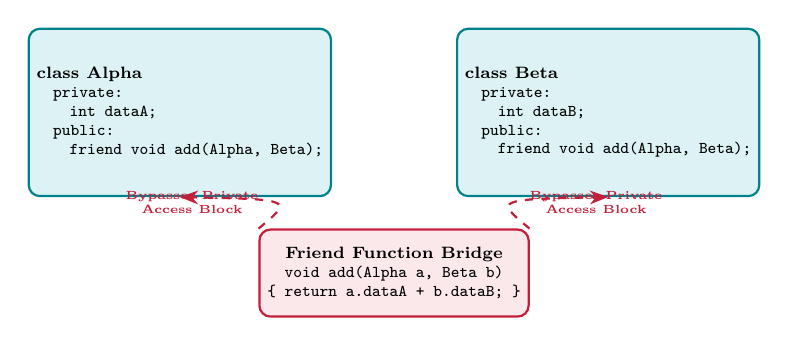
\begin{tikzpicture}[node distance=1.2cm, thick, scale=0.85, every node/.style={scale=0.85}]
  % Class Alpha box
  \node[rectangle, draw=myteal, fill=hdrteal, rounded corners=4pt, minimum width=3.4cm, minimum height=2.5cm, align=left, font=\scriptsize] (classA) at (-3.2, 0) {
    \textbf{class Alpha}\\
    \quad\texttt{private:}\\
    \quad\quad\texttt{int dataA;}\\
    \quad\texttt{public:}\\
    \quad\quad\texttt{friend void add(Alpha, Beta);}
  };

  % Class Beta box
  \node[rectangle, draw=myteal, fill=hdrteal, rounded corners=4pt, minimum width=3.4cm, minimum height=2.5cm, align=left, font=\scriptsize] (classB) at (3.2, 0) {
    \textbf{class Beta}\\
    \quad\texttt{private:}\\
    \quad\quad\texttt{int dataB;}\\
    \quad\texttt{public:}\\
    \quad\quad\texttt{friend void add(Alpha, Beta);}
  };

  % Friend function box (Bridge)
  \node[rectangle, draw=myred, fill=hdrred, rounded corners=4pt, minimum width=4.0cm, minimum height=1.3cm, align=center, font=\scriptsize] (friendFunc) at (0, -2.4) {
    \textbf{Friend Function Bridge}\\
    \texttt{void add(Alpha a, Beta b)}\\
    \texttt{\{ return a.dataA + b.dataB; \}}
  };

  % Path/Bridge
  \draw[arrow, color=myred, dashed, line width=0.8pt] (friendFunc.north west) .. controls (-1.5, -1.3) .. (classA.south) 
    node[midway, left=0.1cm, font=\tiny\bfseries, align=center] {Bypasses Private\\Access Block};
  \draw[arrow, color=myred, dashed, line width=0.8pt] (friendFunc.north east) .. controls (1.5, -1.3) .. (classB.south) 
    node[midway, right=0.1cm, font=\tiny\bfseries, align=center] {Bypasses Private\\Access Block};
\end{tikzpicture}
\end{tcolorbox}

\begin{tcolorbox}[examplebox, title={Code Example: Friend Function accessing private variables of two classes}]
\begin{spacing}{1.0}
\begin{verbatim}
#include <iostream>
class Beta; // Forward declaration required for Alpha's friend prototype

class Alpha {
private:
    int valA;
public:
    Alpha(int v) : valA(v) {}
    friend int add(Alpha, Beta); // Declare friend function
};

class Beta {
private:
    int valB;
public:
    Beta(int v) : valB(v) {}
    friend int add(Alpha, Beta); // Declare same function as friend
};

// Friend function definition (no 'friend' keyword or scope resolution here)
int add(Alpha a, Beta b) {
    return a.valA + b.valB; // Directly accessing private members
}

int main() {
    Alpha a(15);
    Beta b(25);
    std::cout << "Sum = " << add(a, b); // Outputs: Sum = 40
    return 0;
}
\end{verbatim}
\end{spacing}
\end{tcolorbox}

\subsection{Friend Classes}
A class can also be declared as a friend of another class. If \texttt{class B} is declared as a \texttt{friend} inside \texttt{class A}, then \textbf{all} member functions of \texttt{class B} gain access to the private and protected data members of \texttt{class A}.
\begin{equation}
  \texttt{class A \{ friend class B; \}; // Class B is a friend of Class A}
\end{equation}

% ===============================================================================
\section{Object Memory and Dynamic Allocation}
% ===============================================================================

To write efficient code, engineers must understand how objects occupy physical memory and how dynamic memory operators allocate resources on the heap.

\subsection{Memory Considerations for Objects}
When a class is declared, no memory is allocated. Memory is only allocated when objects of that class are instantiated.
\begin{itemize}[leftmargin=*, itemsep=3pt]
  \item \textbf{Data Members:} Each object receives its own independent memory allocation for non-static data members (to hold distinct object states).
  \item \textbf{Member Functions:} Member functions are allocated only once in the \textbf{Code Segment} when the class is loaded. All objects of the class share the exact same memory space for functions. This prevents code redundancy.
\end{itemize}

\begin{tcolorbox}[tikzbox, title={Object Memory Allocation Layout in RAM}]
\centering
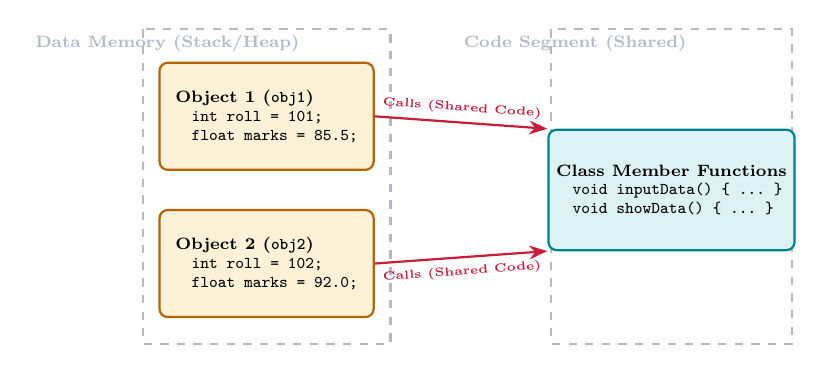
\begin{tikzpicture}[node distance=1.2cm, thick, scale=0.85, every node/.style={scale=0.85}]
  % Stack/Heap (Separate Data Memory)
  \draw[dashed, color=mgframe] (-4.5, 2.2) rectangle (-0.8, -2.5) node[pos=0.1, above, font=\scriptsize\bfseries] {Data Memory (Stack/Heap)};
  
  \node[rectangle, draw=myamber, fill=hdramber, rounded corners=3pt, minimum width=3.2cm, minimum height=1.6cm, align=left, font=\scriptsize] (obj1) at (-2.65, 0.9) {
    \textbf{Object 1 (\texttt{obj1})}\\
    \quad\texttt{int roll = 101;}\\
    \quad\texttt{float marks = 85.5;}
  };
  
  \node[rectangle, draw=myamber, fill=hdramber, rounded corners=3pt, minimum width=3.2cm, minimum height=1.6cm, align=left, font=\scriptsize] (obj2) at (-2.65, -1.3) {
    \textbf{Object 2 (\texttt{obj2})}\\
    \quad\texttt{int roll = 102;}\\
    \quad\texttt{float marks = 92.0;}
  };

  % Code Segment (Shared member functions)
  \draw[dashed, color=mgframe] (1.6, 2.2) rectangle (5.2, -2.5) node[pos=0.1, above, font=\scriptsize\bfseries] {Code Segment (Shared)};
  
  \node[rectangle, draw=myteal, fill=hdrteal, rounded corners=3pt, minimum width=3.2cm, minimum height=1.8cm, align=left, font=\scriptsize] (code) at (3.4, -0.2) {
    \textbf{Class Member Functions}\\
    \quad\texttt{void inputData() \{ ... \}}\\
    \quad\texttt{void showData() \{ ... \}}
  };

  % Arrows representing function invocation
  \draw[arrow, color=myred] (obj1.east) -- (code.north west) node[midway, above, sloped, font=\tiny\bfseries] {Calls (Shared Code)};
  \draw[arrow, color=myred] (obj2.east) -- (code.south west) node[midway, below, sloped, font=\tiny\bfseries] {Calls (Shared Code)};
\end{tikzpicture}
\end{tcolorbox}

\subsection{Dynamic Memory Management: \texorpdfstring{\texttt{new}}{new} and \texorpdfstring{\texttt{delete}}{delete}}
In addition to C's run-time allocation functions (\texttt{malloc}/\texttt{free}), C++ introduces type-safe operators \texttt{new} and \texttt{delete} which operate directly on the Heap memory.

\begin{tcolorbox}[formulabox, title={\textbf{Dynamic Memory Syntax}}]
\begin{align}
  &\text{Allocate Single Variable: } && \texttt{pointer\_var = new data\_type;} \\
  &\text{Allocate Array of Elements: } && \texttt{pointer\_var = new data\_type[size];} \\
  &\text{Deallocate Single Variable: } && \texttt{delete pointer\_var;} \\
  &\text{Deallocate Array: } && \texttt{delete [] pointer\_var;}
\end{align}
\end{tcolorbox}

\textbf{Advantages of \texttt{new}/\texttt{delete} over \texttt{malloc}/\texttt{free}:}
\begin{enumerate}[label=\textbf{\arabic*.}, leftmargin=*, itemsep=2pt]
  \item \textbf{Constructor Calling:} \texttt{new} automatically calls the object's constructor; \texttt{malloc} only allocates raw bytes.
  \item \textbf{Destructor Calling:} \texttt{delete} automatically calls the destructor before freeing memory; \texttt{free} does not.
  \item \textbf{Type Safety:} \texttt{new} returns the exact pointer type (no explicit typecasting needed); \texttt{malloc} returns a \texttt{void*}.
  \item \textbf{Safety:} \texttt{new} throws a \texttt{std::bad\_alloc} exception if allocation fails; \texttt{malloc} returns \texttt{NULL}.
\end{enumerate}

\begin{tcolorbox}[examplebox, title={Code Example: Dynamic allocation of variable and array}]
\begin{spacing}{1.0}
\begin{verbatim}
#include <iostream>
int main() {
    // Dynamic single variable allocation
    int *pInt = new int(42); // Allocates int and initializes to 42
    std::cout << "Value: " << *pInt << std::endl;
    delete pInt; // Free memory

    // Dynamic array allocation
    int size = 5;
    int *arr = new int[size]; // Allocates array of 5 integers
    for (int i = 0; i < size; i++) {
        arr[i] = (i + 1) * 10;
        std::cout << arr[i] << " ";
    }
    std::cout << std::endl;
    
    delete[] arr; // Free array memory (note the square brackets)
    return 0;
}
\end{verbatim}
\end{spacing}
\end{tcolorbox}

% ===============================================================================
% MANDATORY QUICK REVISION PAGE
% ===============================================================================
\newpage
\begin{center}
  {\large\bfseries\color{myred} Quick Revision --- Module III}\\[3pt]
  {\small\color{mydark} Objects and Classes $|$ OE-EC604C}
\end{center}
\noindent{\color{myred}\rule{\linewidth}{1.2pt}}
\vspace{4pt}

\begin{tcolorbox}[formulabox, title={\textbf{Key Syntax and Configurations}}]
\renewcommand{\arraystretch}{1.3}
\begin{tabularx}{\linewidth}{B{3.8cm} X}
Class Declaration        & \texttt{class MyClass \{ private: int x; public: void func(); \};} \\[4pt]
External Definition      & \texttt{void MyClass::func() \{ /* code */ \}} \\[4pt]
Static Definition        & \texttt{int MyClass::staticVar = 0; // Out-of-class definition} \\[4pt]
Friend Declaration       & \texttt{friend void myFriend(MyClass \&obj); // Inside class} \\[4pt]
Dynamic Single           & \texttt{int *ptr = new int(10); \quad delete ptr;} \\[4pt]
Dynamic Array            & \texttt{int *arr = new int[5]; \quad delete [] arr;}
\end{tabularx}
\end{tcolorbox}

\begin{tcolorbox}[defbox, title={\textbf{One-Line Definitions}}]
\begin{itemize}[leftmargin=*, itemsep=2.5pt, topsep=0pt]
  \item \textbf{Class:} A user-defined data type that binds data and functions together into a single unit.
  \item \textbf{Object:} An instance of a class that represents a real-world entity and occupies memory.
  \item \textbf{Access Specifiers:} Keywords (\texttt{private}, \texttt{public}, \texttt{protected}) that define the accessibility of class members.
  \item \textbf{Static Data Member:} A class variable shared by all class objects, residing in global static memory.
  \item \textbf{Static Member Function:} A function that can only access static members and is called without an object.
  \item \textbf{Friend Function:} A non-member function declared inside a class that can access its private and protected members.
  \item \textbf{Friend Class:} A class whose member functions can all access the private and protected members of another class.
  \item \textbf{new Operator:} A C++ operator used to dynamically allocate memory on the heap and run constructors.
  \item \textbf{delete Operator:} A C++ operator used to release dynamically allocated heap memory and run destructors.
\end{itemize}
\end{tcolorbox}

\begin{tcolorbox}[exambox, title={\textbf{Frequently Asked / Viva Questions}}]
\begin{enumerate}[topsep=0pt, label=\textbf{Q\arabic*.}, itemsep=5pt]
  \item \Q{What is the default access specifier for class members in C++?}
    The default access specifier is \texttt{private}. If no access specifier is mentioned, members are treated as private.
  \item \Q{Why do member functions defined inside the class run faster than those defined outside?}
    Member functions defined inside the class are implicitly treated as \texttt{inline}, meaning the compiler attempts to substitute the call site with the function code, avoiding call overhead.
  \item \Q{Why must static data members be defined outside the class scope?}
    The class declaration only defines the type, it does not allocate memory. Defining it outside allocates physical storage in global memory.
  \item \Q{Can a static member function access non-static variables of the class?}
    No. A static function is not bound to any object instance, so it lacks a \texttt{this} pointer and cannot determine which object's non-static variable to access.
  \item \Q{Explain why a friend function cannot be called using the object dot (.) operator.}
    A friend function is not a member of the class. It is a normal global function with special access rights, so calling it with \texttt{obj.} causes a compile error.
  \item \Q{Does declaring a friend function inside a class violate encapsulation?}
    Theoretically yes, as it bypasses private access blocks. However, it is controlled by the class designer and is useful for operations like operator overloading.
  \item \Q{What is the memory size of an empty class object in C++?}
    It is 1 byte. The compiler allocates 1 byte to ensure that two different object instances of the empty class have unique memory addresses.
  \item \Q{What happens if you use \texttt{delete} instead of \texttt{delete []} to free a dynamically allocated array?}
    It results in undefined behavior. Typically, the compiler will only call the destructor for the first element in the array and may fail to release the entire block of memory.
  \item \Q{What is the difference between class and struct in C++?}
    In a \texttt{struct}, members are \texttt{public} by default, whereas in a \texttt{class}, members are \texttt{private} by default.
  \item \Q{Can we declare a constructor static in C++?}
    No. Constructors are called to initialize specific object instances. A static function has no instance binding, making a static constructor logically impossible.
  \item \Q{Does \texttt{new} return a void pointer like \texttt{malloc}?}
    No. The \texttt{new} operator is type-safe and returns a typed pointer to the allocated memory, eliminating the need for casting.
  \item \Q{Can we overload a friend function?}
    Yes, a friend function is a regular function and can be overloaded like any other non-member function.
\end{enumerate}
\end{tcolorbox}

\begin{tcolorbox}[tikzbox, title={Comparison: C++ dynamic operators vs. C memory functions}]
\renewcommand{\arraystretch}{1.45}
\par\noindent
\begin{tabularx}{\linewidth}{|B{3.2cm}|Y|Y|}
\hline
\textbf{Feature} & \textbf{\color{myteal}new / delete (C++)} & \textbf{\color{myamber}malloc / free (C)} \\
\hline
\textbf{Type Safety} & Type-safe; returns exact type pointer. & Returns \texttt{void*}; requires explicit typecasting. \\
\hline
\textbf{Constructors} & Calls constructors automatically for classes. & Does not trigger constructors (allocates raw bytes). \\
\hline
\textbf{Destructors} & Calls destructors automatically. & Does not trigger destructors. \\
\hline
\textbf{Failure Behavior} & Throws \texttt{std::bad\_alloc} exception. & Returns \texttt{NULL}. \\
\hline
\textbf{Buffer Size} & Automatically calculated by compiler. & Must be explicitly calculated in bytes using \texttt{sizeof}. \\
\hline
\end{tabularx}
\end{tcolorbox}

\end{document}
